\section{Experiment design}\label{sec:experiment_design}
%Forsoegsopstilling, der inkludere en tegning af omraadet set oppefra med indtegning af beacons, objectern og hvor rigtige position for test person.
Experiments for the evaluation of the implemented system are carried out in an $4.75m \times 6.5m$ meeting room.
In the room, a partition and a cabinet are placed between two tables, effectively dividing a single meeting room into two smaller areas. 
In each of the smaller areas a table with six chairs is placed and on the walls are placed whiteboards.
\begin{figure}[h]
    \centering
    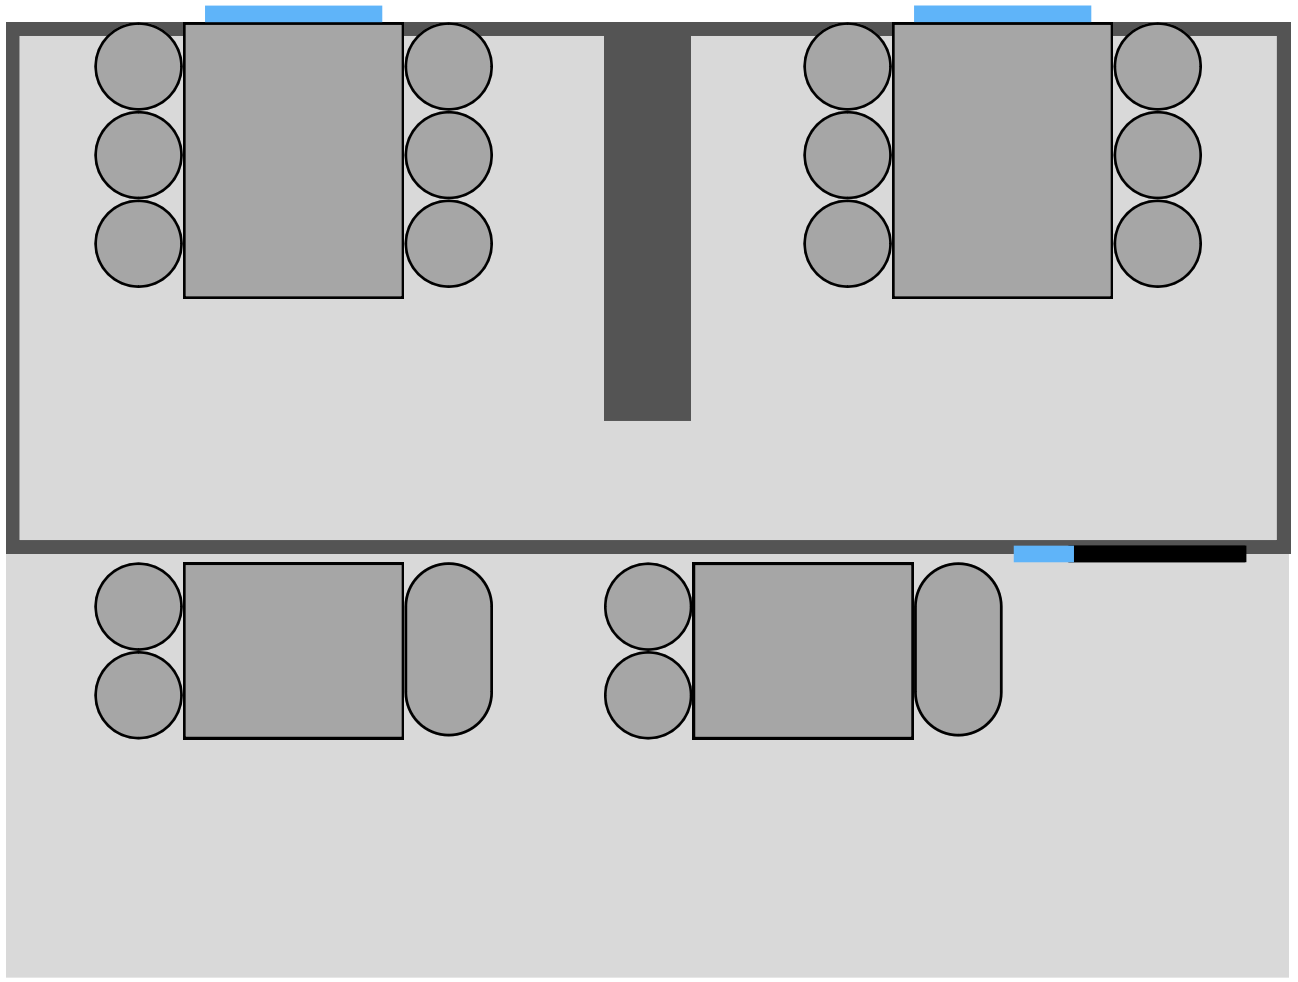
\includegraphics[scale=0.7]{images/experiment_room.png}
    \caption{A sketch of the meeting room in which the experiments were carried out.}
    \label{fig:experiment_room}
\end{figure}
On one end of each table is a large, rectangular window.
Furthermore, one table has a large TV screen placed near the window. 
Near the door of the room, an airconditioning controller and a large glass window are located.
Lighting is built into the ceiling, thus no hanging light will interfere with the broadcasted signals. 
Outside the meeting room is a common area.
This area contains two high tables.
Each of these tables has a small couch and two chairs placed next to it.
Beacons are placed on top of the cabinet and in the three corners furthest away from the door.   
The meeting room and its surrounding area is depicted in Figure \ref{fig:experiment_room}.


\subsection{Creating a map}
To execute the first phase of the approach described in Section \label{sec:first_phase}, we first partition the previously described meeting room into a $1m \times 1m$ resolutionn grid and place beacons.
To perform measurements inside each cell of the grid, a person holding a phone traverses systematically through the room and stops in each cell to collect data. 
We will refer to this person as a \textit{collector}.
The data is collected using a smart-phone, with a developed app installed.   \todo{do we need to describe this in depth somewhere? NEED TO DESCRIBE THE APP SOMEWHERE}
With the app, it is possible to perform measurements from any number of selected beacons and append a label to the measurements.
\begin{figure}[h]
    \centering
    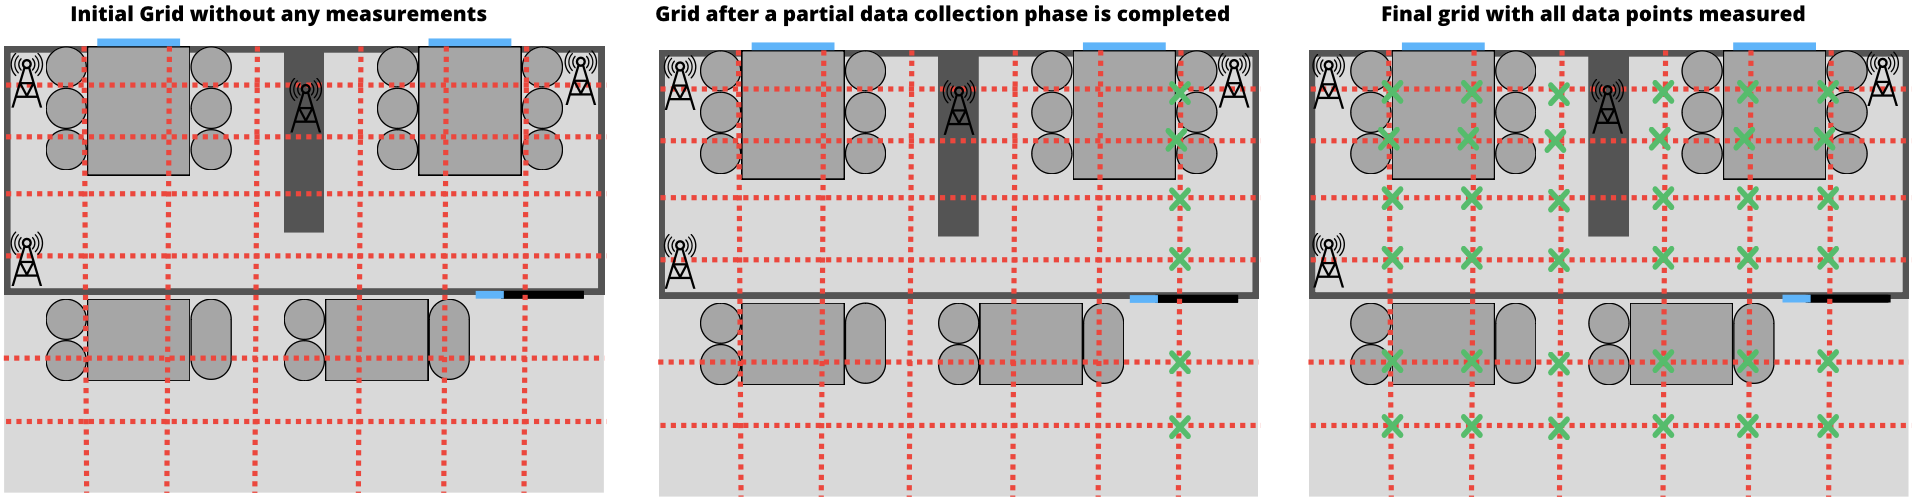
\includegraphics[width=\textwidth]{images/experiment_map_creation.png}
    \caption{A sketch of the meeting room partitioned into a grid decorated with beacon placements (red antenna) and measurement locations (green cross). The figure how the measurements are collected systematically in the meeting room.}
    \label{fig:experiment_map_creation}
\end{figure}

When the collector stops in a cell, they can press a button in the app, which starts measuring after n seconds. \todo{figure out how many seconds we need}
The phone provides auditory feedback when it has collected enough adverticements for the requirements described in Section \ref{sec:first_phase} to be fulfilled.
When the information for the cell has been computed and stored on the phone, the collector is informed and continues to the next cell in the grid. 
During the measurement the phone is kept in roughly the same height.
Measurements are collected in a setup using 4 beacons, as depicted in Figure \ref{fig:experiment_map_creation}.

\subsection{Evaluation strategy}
\begin{figure}[h]
    \centering
    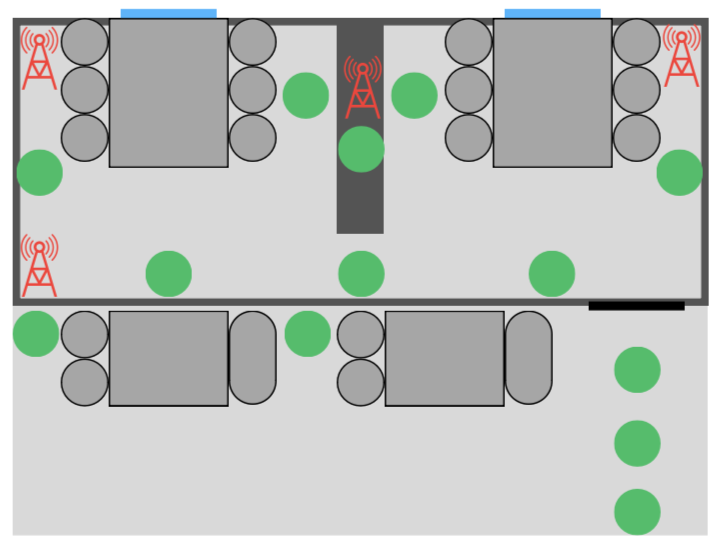
\includegraphics[scale=0.7]{images/experiment_setup.png}
    \caption{A sketch of the meeting room in which the experiments were carried out, decorated with beacon placements (red antenna) and measurement locations(green circles)}
    \label{fig:experiment_setup}
\end{figure}
When performing the evaluations, we want to examine whether the system can correctly classify whether a receiving device is inside the room.
We do this by performing measurements inside, outside, and on borders of the room.
As physical obstacles can cause fluctuations in the received signals, we design the expirement such that measurements are takens in areas where some, none, and all of the beacons are blocked. 
We perform measurements in the following areas:
\begin{itemize}
    \item Along the walls inside of the meeting room
    \item Along both sides of the divider
    \item On the cabinet, next to the beacon
    \item 1m, 2m, 3m outside the door   
    \item By the tables in the common area. 
\end{itemize}
Data collection points and beacon placement of the room during the experiment is seen in Figure \ref{fig:experiment_setup}.


\todo{we should describe that we perform these test on x devices (specific devices) and maybe run the test multiple times with small changes to the environment(not beacon placement), for instance placing computers or devices that create noise.}